\documentclass{standalone}
\usepackage{tikz}
\usetikzlibrary{patterns, positioning}

\begin{document}
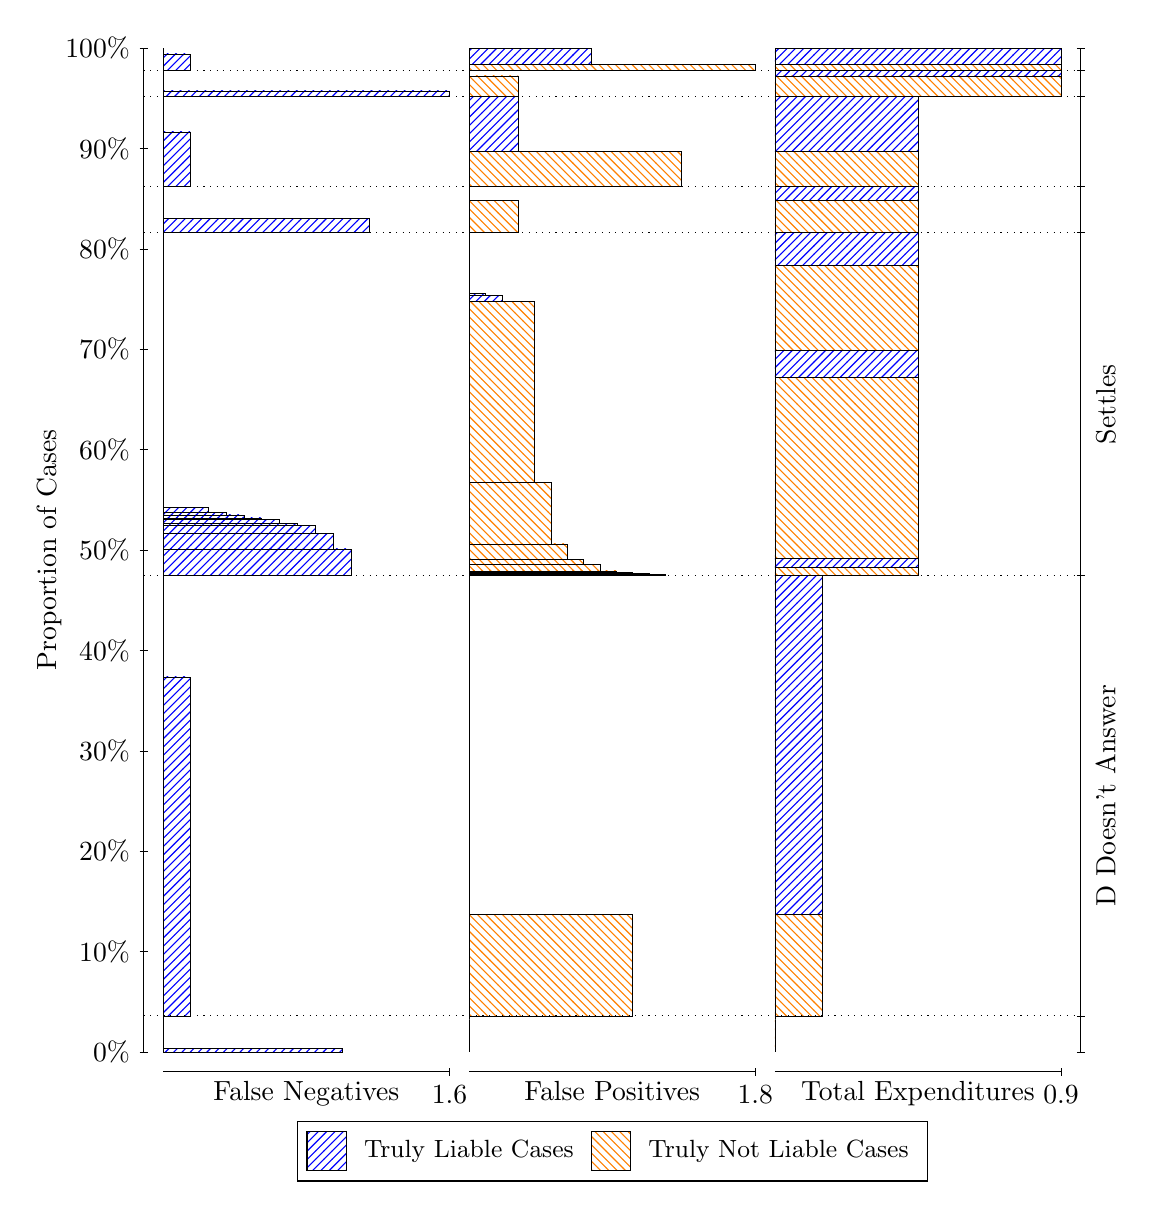
\begin{tikzpicture}
\draw[black, very thin] (1.5,1.75) -- (1.5,14.5);
\node[rotate=90, anchor=center] at (0.3, 8.125) {Proportion of Cases};
\draw[black, very thin] (1.45,1.75) -- (1.55,1.75);
\node[anchor=east] at (1.45, 1.75) {0\%};
\draw[black, very thin] (1.45,3.025) -- (1.55,3.025);
\node[anchor=east] at (1.45, 3.025) {10\%};
\draw[black, very thin] (1.45,4.3) -- (1.55,4.3);
\node[anchor=east] at (1.45, 4.3) {20\%};
\draw[black, very thin] (1.45,5.575) -- (1.55,5.575);
\node[anchor=east] at (1.45, 5.575) {30\%};
\draw[black, very thin] (1.45,6.85) -- (1.55,6.85);
\node[anchor=east] at (1.45, 6.85) {40\%};
\draw[black, very thin] (1.45,8.125) -- (1.55,8.125);
\node[anchor=east] at (1.45, 8.125) {50\%};
\draw[black, very thin] (1.45,9.4) -- (1.55,9.4);
\node[anchor=east] at (1.45, 9.4) {60\%};
\draw[black, very thin] (1.45,10.675) -- (1.55,10.675);
\node[anchor=east] at (1.45, 10.675) {70\%};
\draw[black, very thin] (1.45,11.95) -- (1.55,11.95);
\node[anchor=east] at (1.45, 11.95) {80\%};
\draw[black, very thin] (1.45,13.225) -- (1.55,13.225);
\node[anchor=east] at (1.45, 13.225) {90\%};
\draw[black, very thin] (1.45,14.5) -- (1.55,14.5);
\node[anchor=east] at (1.45, 14.5) {100\%};

\draw[black, very thin] (13.4,1.75) -- (13.4,14.5);
\draw[black, very thin] (13.35,1.75) -- (13.45,1.75);
\node[anchor=west] at (13.35, 1.75) {};
\draw[black, very thin] (13.35,2.208) -- (13.45,2.208);
\node[anchor=west] at (13.35, 2.208) {};
\draw[black, very thin] (13.35,7.799) -- (13.45,7.799);
\node[anchor=west] at (13.35, 7.799) {};
\draw[black, very thin] (13.35,12.155) -- (13.45,12.155);
\node[anchor=west] at (13.35, 12.155) {};
\draw[black, very thin] (13.35,12.744) -- (13.45,12.744);
\node[anchor=west] at (13.35, 12.744) {};
\draw[black, very thin] (13.35,13.881) -- (13.45,13.881);
\node[anchor=west] at (13.35, 13.881) {};
\draw[black, very thin] (13.35,14.22) -- (13.45,14.22);
\node[anchor=west] at (13.35, 14.22) {};
\draw[black, very thin] (13.35,14.5) -- (13.45,14.5);
\node[anchor=west] at (13.35, 14.5) {};

\draw[black, very thin, pattern color=blue, pattern=north east lines] (1.75,1.75) rectangle (4.0208,1.7982);
\draw[black, very thin, pattern color=orange, pattern=north west lines] (1.75,1.7982) rectangle (1.75,2.208);
\draw[black, very thin, pattern color=blue, pattern=north east lines] (1.75,2.208) rectangle (2.0906,6.5142);
\draw[black, very thin, pattern color=orange, pattern=north west lines] (1.75,6.5142) rectangle (1.75,7.799);
\draw[black, very thin, pattern color=blue, pattern=north east lines] (1.75,7.799) rectangle (4.1344,8.1381);
\draw[black, very thin, pattern color=blue, pattern=north east lines] (1.75,8.1381) rectangle (3.9073,8.3326);
\draw[black, very thin, pattern color=blue, pattern=north east lines] (1.75,8.3326) rectangle (3.6802,8.4339);
\draw[black, very thin, pattern color=blue, pattern=north east lines] (1.75,8.4339) rectangle (3.4531,8.4673);
\draw[black, very thin, pattern color=blue, pattern=north east lines] (1.75,8.4673) rectangle (3.226,8.5103);
\draw[black, very thin, pattern color=blue, pattern=north east lines] (1.75,8.5103) rectangle (2.999,8.5317);
\draw[black, very thin, pattern color=blue, pattern=north east lines] (1.75,8.5317) rectangle (2.7719,8.5703);
\draw[black, very thin, pattern color=blue, pattern=north east lines] (1.75,8.5703) rectangle (2.5448,8.5999);
\draw[black, very thin, pattern color=blue, pattern=north east lines] (1.75,8.5999) rectangle (2.3177,8.6671);
\draw[black, very thin, pattern color=orange, pattern=north west lines] (1.75,8.6671) rectangle (1.75,12.155);
\draw[black, very thin, pattern color=blue, pattern=north east lines] (1.75,12.155) rectangle (4.3615,12.335);
\draw[black, very thin, pattern color=orange, pattern=north west lines] (1.75,12.335) rectangle (1.75,12.744);
\draw[black, very thin, pattern color=blue, pattern=north east lines] (1.75,12.744) rectangle (2.0906,13.436);
\draw[black, very thin, pattern color=orange, pattern=north west lines] (1.75,13.436) rectangle (1.75,13.881);
\draw[black, very thin, pattern color=blue, pattern=north east lines] (1.75,13.881) rectangle (5.3833,13.955);
\draw[black, very thin, pattern color=orange, pattern=north west lines] (1.75,13.955) rectangle (1.75,14.22);
\draw[black, very thin, pattern color=blue, pattern=north east lines] (1.75,14.22) rectangle (2.0906,14.426);
\draw[black, very thin, pattern color=orange, pattern=north west lines] (1.75,14.426) rectangle (1.75,14.5);
\draw[black, very thin, pattern color=orange, pattern=north west lines] (5.6333,1.75) rectangle (5.6333,2.1599);
\draw[black, very thin, pattern color=blue, pattern=north east lines] (5.6333,2.1599) rectangle (5.6333,2.208);
\draw[black, very thin, pattern color=orange, pattern=north west lines] (5.6333,2.208) rectangle (7.7095,3.4928);
\draw[black, very thin, pattern color=blue, pattern=north east lines] (5.6333,3.4928) rectangle (5.6333,7.799);
\draw[black, very thin, pattern color=orange, pattern=north west lines] (5.6333,7.799) rectangle (8.1248,7.8138);
\draw[black, very thin, pattern color=orange, pattern=north west lines] (5.6333,7.8138) rectangle (7.9171,7.8243);
\draw[black, very thin, pattern color=orange, pattern=north west lines] (5.6333,7.8243) rectangle (7.7095,7.8409);
\draw[black, very thin, pattern color=orange, pattern=north west lines] (5.6333,7.8409) rectangle (7.5019,7.8597);
\draw[black, very thin, pattern color=orange, pattern=north west lines] (5.6333,7.8597) rectangle (7.2943,7.9386);
\draw[black, very thin, pattern color=orange, pattern=north west lines] (5.6333,7.9386) rectangle (7.0867,8.008);
\draw[black, very thin, pattern color=orange, pattern=north west lines] (5.6333,8.008) rectangle (6.879,8.2038);
\draw[black, very thin, pattern color=orange, pattern=north west lines] (5.6333,8.2038) rectangle (6.6714,8.9812);
\draw[black, very thin, pattern color=orange, pattern=north west lines] (5.6333,8.9812) rectangle (6.4638,11.287);
\draw[black, very thin, pattern color=blue, pattern=north east lines] (5.6333,11.287) rectangle (6.0486,11.354);
\draw[black, very thin, pattern color=blue, pattern=north east lines] (5.6333,11.354) rectangle (5.841,11.384);
\draw[black, very thin, pattern color=blue, pattern=north east lines] (5.6333,11.384) rectangle (5.6333,12.155);
\draw[black, very thin, pattern color=orange, pattern=north west lines] (5.6333,12.155) rectangle (6.2562,12.564);
\draw[black, very thin, pattern color=blue, pattern=north east lines] (5.6333,12.564) rectangle (5.6333,12.744);
\draw[black, very thin, pattern color=orange, pattern=north west lines] (5.6333,12.744) rectangle (8.3324,13.189);
\draw[black, very thin, pattern color=blue, pattern=north east lines] (5.6333,13.189) rectangle (6.2562,13.881);
\draw[black, very thin, pattern color=orange, pattern=north west lines] (5.6333,13.881) rectangle (6.2562,14.146);
\draw[black, very thin, pattern color=blue, pattern=north east lines] (5.6333,14.146) rectangle (5.6333,14.22);
\draw[black, very thin, pattern color=orange, pattern=north west lines] (5.6333,14.22) rectangle (9.2667,14.294);
\draw[black, very thin, pattern color=blue, pattern=north east lines] (5.6333,14.294) rectangle (7.1905,14.5);
\draw[black, very thin, pattern color=orange, pattern=north west lines] (9.5167,1.75) rectangle (9.5167,2.1599);
\draw[black, very thin, pattern color=blue, pattern=north east lines] (9.5167,2.1599) rectangle (9.5167,2.208);
\draw[black, very thin, pattern color=orange, pattern=north west lines] (9.5167,2.208) rectangle (10.122,3.4928);
\draw[black, very thin, pattern color=blue, pattern=north east lines] (9.5167,3.4928) rectangle (10.122,7.799);
\draw[black, very thin, pattern color=orange, pattern=north west lines] (9.5167,7.799) rectangle (11.333,7.9049);
\draw[black, very thin, pattern color=blue, pattern=north east lines] (9.5167,7.9049) rectangle (11.333,8.0162);
\draw[black, very thin, pattern color=orange, pattern=north west lines] (9.5167,8.0162) rectangle (11.333,10.322);
\draw[black, very thin, pattern color=blue, pattern=north east lines] (9.5167,10.322) rectangle (11.333,10.661);
\draw[black, very thin, pattern color=orange, pattern=north west lines] (9.5167,10.661) rectangle (11.333,11.737);
\draw[black, very thin, pattern color=blue, pattern=north east lines] (9.5167,11.737) rectangle (11.333,12.155);
\draw[black, very thin, pattern color=orange, pattern=north west lines] (9.5167,12.155) rectangle (11.333,12.564);
\draw[black, very thin, pattern color=blue, pattern=north east lines] (9.5167,12.564) rectangle (11.333,12.744);
\draw[black, very thin, pattern color=orange, pattern=north west lines] (9.5167,12.744) rectangle (11.333,13.189);
\draw[black, very thin, pattern color=blue, pattern=north east lines] (9.5167,13.189) rectangle (11.333,13.881);
\draw[black, very thin, pattern color=orange, pattern=north west lines] (9.5167,13.881) rectangle (13.15,14.146);
\draw[black, very thin, pattern color=blue, pattern=north east lines] (9.5167,14.146) rectangle (13.15,14.22);
\draw[black, very thin, pattern color=orange, pattern=north west lines] (9.5167,14.22) rectangle (13.15,14.294);
\draw[black, very thin, pattern color=blue, pattern=north east lines] (9.5167,14.294) rectangle (13.15,14.5);
\draw[black, dotted] (1.5,2.208) -- (13.4,2.208);
\draw[black, dotted] (1.5,7.799) -- (13.4,7.799);
\draw[black, dotted] (1.5,12.155) -- (13.4,12.155);
\draw[black, dotted] (1.5,12.744) -- (13.4,12.744);
\draw[black, dotted] (1.5,13.881) -- (13.4,13.881);
\draw[black, dotted] (1.5,14.22) -- (13.4,14.22);
\draw[black, very thin] (1.75,1.5) -- (5.3833,1.5);
\node[anchor=north] at (3.5667, 1.5) {False Negatives};
\draw[black, very thin] (5.3833,1.45) -- (5.3833,1.55);
\node[anchor=north] at (5.3833, 1.45) {1.6};

\draw[black, very thin] (5.6333,1.5) -- (9.2667,1.5);
\node[anchor=north] at (7.45, 1.5) {False Positives};
\draw[black, very thin] (9.2667,1.45) -- (9.2667,1.55);
\node[anchor=north] at (9.2667, 1.45) {1.8};

\draw[black, very thin] (9.5167,1.5) -- (13.15,1.5);
\node[anchor=north] at (11.333, 1.5) {Total Expenditures};
\draw[black, very thin] (13.15,1.45) -- (13.15,1.55);
\node[anchor=north] at (13.15, 1.45) {0.9};


\node[black, centered, rotate=90] at (13.72, 5.0035) {D Doesn't Answer};
\node[black, centered, rotate=90] at (13.72, 9.9771) {Settles};





\draw (7.449999999999999,1.5) node[draw=none] (baseCoordinate) {};
\begin{scope}[align=center]
        \matrix[scale=0.5, draw=black, below=0.5cm of baseCoordinate, nodes={draw}, column sep=0.1cm]{
            \node[rectangle, draw, minimum width=0.5cm, minimum height=0.5cm, pattern=north east lines, pattern color=blue] {}; &
            \node[draw=none, font=\small] (B) {Truly Liable Cases}; &
            \node[rectangle, draw, minimum width=0.5cm, minimum height=0.5cm, pattern=north west lines, pattern color=orange] {}; &
            \node[draw=none, font=\small] (B) {Truly Not Liable Cases}; \\
            };
\end{scope}

\end{tikzpicture}
\end{document}